\documentclass[openany]{UoYCSproject}

\protect\BEng
\protect\supervisor{Dr William Smith}
\protect\wordcount{(to-be-completed)}
\protect\includes{the title page, abstract and body of the report}
\protect\excludes{bibliographies and appendices}
\protect\abstract{This project produces a functional mobile application to visualise potential avalanche hazards along popular winter mountaineering routes within a 3D terrain reality, with a primary focus on Scottish mountains while providing excellent adaptability for other regions with appropriate data sources. Avalanche hazards were projected from a combination of professional avalanche forecasts and spatial analysis of mountain terrain models. Both the accuracy and the usability of the application were evaluated through various methods. The safety and ethical considerations on the application being put into real world use were also discussed.}

\usepackage[left=26mm,top=26mm,right=26mm,bottom=26mm]{geometry}    
\geometry{a4paper}                   		
\usepackage{graphicx}					
\usepackage{amssymb}
\usepackage{url}
\usepackage[parfill]{parskip}
\usepackage{natbib}
\setlength{\headsep}{5pt}
\graphicspath{ {images/} }
\setlength{\bibsep}{3pt plus 3ex}

\title{An App for Visualisation of Avalanche Hazard}
\author{Chongyang Shi}
\date{(to-be-completed)}							
\begin{document}

{\let\cleardoublepage\clearpage 
    \maketitle
}

\chapter{Introduction}

\section{Overview of the project}

The purpose of this project is to produce a functional mobile application to visualise potential avalanche hazards along popular winter mountaineering routes within a 3D terrain reality, with a primary focus on Scottish mountains while providing excellent adaptability for other regions with appropriate data sources. 

A model for projecting localised avalanche hazards based on carefully sourced and processed avalanche forecasts \cite{sais} and terrain model data \cite{os-5} was produced by the project. The accuracy of the model has been evaluated against past avalanche records \cite[pp. 143-151]{scottish-avalanches}\cite{sais-map}. Usability and effectiveness of the application guiding the user away from hazardous locations were evaluated through experiments and test uses conducted with experienced mountaineers.

The project incorporated tools and techniques from various aspects of Computer Science, including software engineering, geographic information system (GIS) modelling, human-computer interaction, computer graphics and algorithms. Many of these tools and techniques are associated with current research in these areas.

\section{Motivations behind the application}

As a front-runner of digital avalanche forecasts, the Scottish Avalanche Information Service \cite{sais} have been providing frequent and reliable winter avalanche forecasts for decades in Scotland.

In addition to written observations on conditions of the snowpack and weather, a typical SAIS avalanche forecast also includes a compass ross, providing avalanche risk levels on the scale of 1 to 5 for slopes of different aspects above and below a transition threshold altitude, shown in \ref{fig:mapping}. However, while this compass rose provides a comprehensive overview on avalanche risks across the forecast region, it is not straightforward to interpret, as the user will need to work out the surface aspects and altitudes along their route, and mentally infer the risk levels of different locations along their route. This is a very complex task, and prone to errors as risk levels could vary sharply between neighbouring aspects and altitudes, as shown in \ref{fig:mapping}.

\begin{figure}[h]
		\centering
		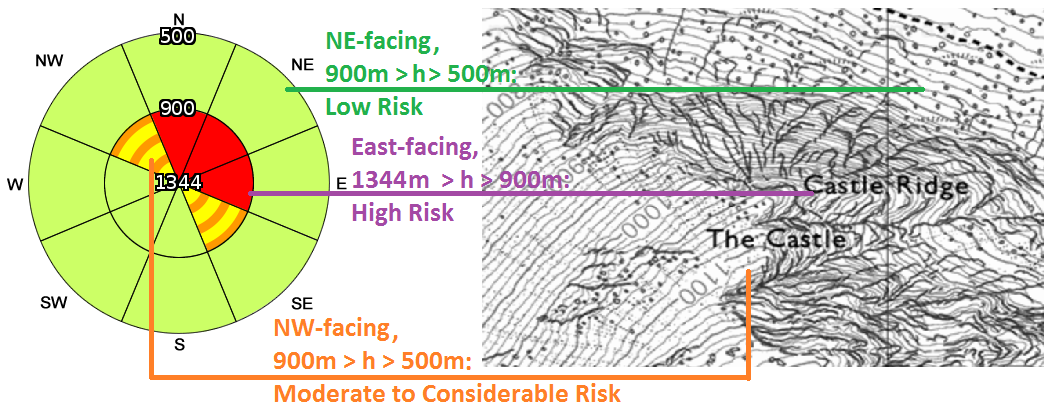
\includegraphics[scale=1]{Mapping.png}
		\caption{\label{fig:mapping} An example compass rose produced by the SAIS on Jan 1, 2016 for Lochaber (left), showing a steep transition of risk levels; and an example manual inference of risk levels based on the compass ross and contour lines near Ben Nevis, Lochaber (right).  \cite{sais-lochaber0106}}
\end{figure}

Therefore, the primary purpose of this project is to vastly simply this process, by generating a coloured image based on the altitude and surface aspects at each point (as determined by a terrain raster model), which is then laid on top of a computer-generated terrain model in the 3D terrain viewer. Hence the information supplied by the compass rose can be visualised in the most straightforward way, allowing the user to freely navigate the 3D model and observe the hazard levels at each location along their route. 

In later stages of the project, we also seek to improve hazard representation through constructing a custom risk model based on information from the compass rose and terrain spatial data; and to improve the functionalities of the application by adding in features such as pathfinding.

\section{Stages of the project}

The course of the project was divided into four development and evaluation stages, in order to effectively track and manage the workload. As the product from each stage is able to function independently of work done in other stages, risks from unforeseen difficulties encountered in research and development can be effectively mitigated. The four stages are described as followed:

\textbf{Stage 1 - Basic Functionalities:} The aim of this stage was to select an appropriate application framework and libraries to produce a basic but functional application -- a 3D terrain viewer with a hazard map overlay, the data for which would be derived solely from forecasts by the Scottish Avalanche Information Service \cite{sais}. The WebGL framework Cesium \cite{cesium} was chosen as the foundation for front-end developments, while Python was chosen to be used to develop the backend, and to interface other systems such as GIS processors with its vast range of interfacing libraries. A functional product was delivered for this stage in early November, 2016.

\textbf{Stage 2 - Improved Spatial Analysis and Evaluation:} This stage of the project expands the data source for generating the hazard map overlay by performing surface fitting and spatial analysis on the terrain model data \cite{os-5}, in order to make the hazards more localised, and to better reflect the hazard posed by unique terrain features such as concave slopes. MATLAB \cite{matlab-primer} was used to perform the computations for these purposes. Evaluations on the localised hazard map against avalanche records were also conducted at this stage, with a focus on the avalanche ``blackspots'' of Scottish mountains.

\textbf{Stage 3 - Pathfinding and Risk Calculator:} With a localised hazard map obtained in Stage 2, this stage was focused on developing a pathfinding tool for the front end application, allowing the user to plot a potential hiking path with a configurable avalanche risk level. Techniques such as A* path finding \cite{cui2011based} were utilised to develop this functionality. 

\textbf{Stage 4 - Usability Testing:} The final stage of the project focus on the human-computer interaction aspects of the application. Experienced mountaineers were consulted and invited to test use the application to provide feedbacks on usability, as well as the effectiveness of the application guiding them away from avalanches that would have occurred in real use. Some improvements were made based on the feedbacks.

\section{Considerations and statements on ethics}

The application was designed as a tool to improve winter mountaineering safety, therefore evidently the foremost consideration on ethics regarding the accuracy and robustness of avalanche hazards projected by the application. If a location with imminent avalanche threat is reported as safe by the application, a user relying on the guidance of this application could be placed in serious danger; conversely, if the application indicate avalanche warnings to users at a location where an avalanche is unlikely to occur, undue anxiety could be caused.

Due to the constraints placed on this project, it is difficult to conduct an extensive peer review process to examine the accuracy of hazard projections. And while most open source libraries utilised during the development process have been widely-used and well-tested, software errors may still occur and affect the safety assurance of the product. Furthermore, the lack of a known commercial or academic product with comparable functionalities eliminates the possibilities of cross-testing the software product.

As a result, while the application is functional and showed promise during our own evaluations, it is not considered as a product ready for real-life use -- a warning of which is displayed when a user initially accesses the application.

\section{Structure of this report}

A literature review is conducted in Chapter \ref{ch:lit-review} over existing research and developments in the various aspects of Computer Science involved in this project. The procurement and processing of both avalanche forecast and topographical data used across all stages of the project are discussed in Chapter \ref{ch:data}. Chapter \ref{ch:app-description} describes in detail the features and internal architectures of the application, as well as its development process. This is followed by Chapter \ref{ch:app-testing}, which describes the evaluation and testing conducted on the application and the quality of its data, mainly conducted during \textbf{Stage 4}. Finally, Chapter \ref{ch:conclusions} concludes the report and discusses the potential uses and future developments of the application.

\chapter{Literature Review} \label{ch:lit-review}

\section{Avalanche forecasting and related researches}

Snow avalanches occur when large masses of snow or ice move rapidly down a mountainside or over a precipice, often triggered from the snow cover \cite[p. 1]{91097820150101}. Avalanches can either be triggered naturally due to certain combinations of geographical \cite[p. 17]{91097820150101} and meteorological \cite[p. 23]{91097820150101} conditions, or triggered by human activities nearby \cite{schweizer2001characteristics}. Regardless of triggering source, avalanches are often deadly to human present nearby, especially when travelling outside areas with built-up defense \cite{91097820150101}, as it often occurs to mountaineers. During the 45 years leading up to 1999, a total of 440 fatalities from avalanche incidents were recorded in the United States \cite{PAGE1999146}; where in the UK, Scottish mountain avalanches alone claimed tens of lives during the same time period \cite{scottish-avalanches}.

With a prosperous winter sport industry bringing millions to mountains and resorts every year\cite{hudson2003sport}, accurate forecasting of avalanches is becoming increasingly critical. Avalanche forecasting is defined as predictions of current and future snow instability in space and time relative to a given triggering level for avalanche initiation \cite[p. 131]{McClung2002}. When applied, the main concerns of such predictions are of risk to humans or property. 

While historically forecasting had been mainly conducted through observations by experienced meteorologists and mountain guides, the vast increase in accessible computing power since the 1990s has provided broad opportunities of applying computation models in avalanche forecasting, as McClung \cite{McClung1994}. has explored as early as in 1994. Numerous models have since been developed, including a snow profile comparison method by Lehning \textit{et al.} \cite{Lehning2001253} and later improved by Hirashima \textit{et al.} in 2007; as well as a method based on observations of tree-rings by Christophe \textit{et al.} \cite{Christophe2010107}. However, the most widely used method -- the Nearest Neighbour (NN) method was initially developed by Buser \cite{buser1983avalanche} in 1983, which has been improved and supplemented by various studies, such as Purves \textit{et al.} in 2003, and Singh and Ganju \cite{Singh2004105} \cite{Singh201533} since 2004.

The most notable application of the NN method is by the Scottish Avalanche Information Service (SAIS) \cite{sais}, which is a government agency responsible for providing daily avalanche information and forecasts of major Scottish mountain attractions during the winter sports season. Avalanche forecasts from the SAIS achieved a weighted accuracy of between 71\% and 82\% on visible winter days between 1988 and 2002 \cite[p. 351] {Purves2003343}. With up to 205 avalanches reported by mountaineers during the winter season of 2015-2016 \cite{sais} (as partly shown in Figure \ref{fig:scotava1516}), the SAIS plays a very significant role in saving lives from avalanches. The SAIS forecasts would also be a major influence factor in data processing and imagery generation of this project.

\begin{figure}[h]
		\centering
		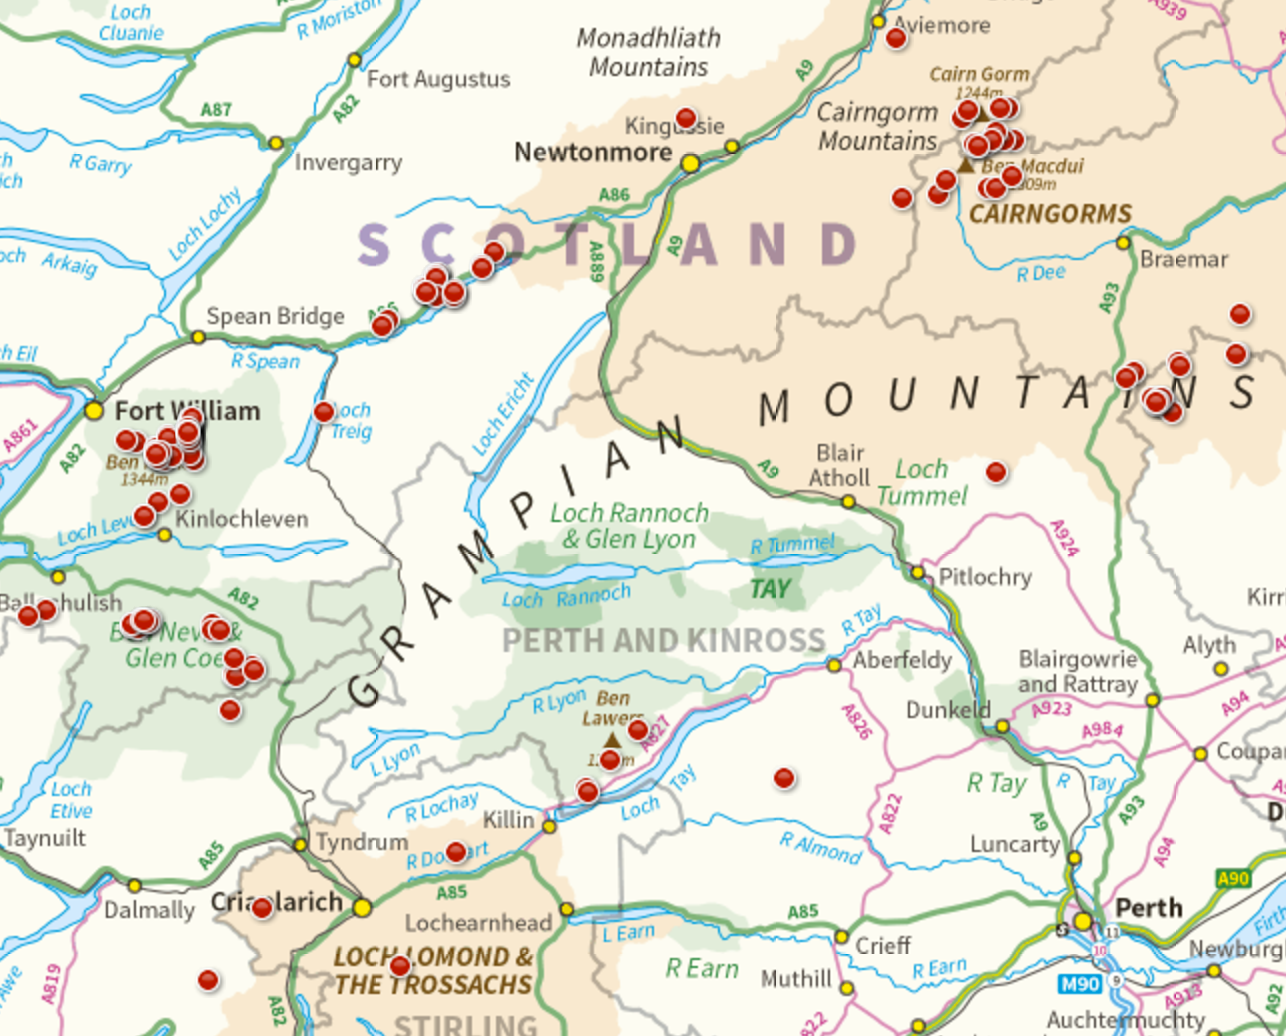
\includegraphics[scale=0.4]{ScotAvalanches1516.png}
		\caption{\label{fig:scotava1516} User-reported avalanches in the Cairngorms and the Glencoe regions during winter sports season of 2015-2016, produced by the SAIS.\cite{sais-map}}
\end{figure}


\chapter{Procurement and Processing of Data} \label{ch:data}

\chapter{Description of the Application} \label{ch:app-description}

\chapter{Evaluation and Testing of the Application} \label{ch:app-testing}

\chapter{Conclusions} \label{ch:conclusions}

\small{\bibliography{project}}
\end{document}  